\section{ Bearbeitung }\label{se:method}

\subsection*{ Zu Teilaufgabe a }
\paragraph*{}
Zunächst müssen die Grenzen bestimmt werden, in denen sich die Parameter $\alpha_i$ bewegen dürfen.
Damit A* und IDA* korrekt arbeiten, muss die verwendete heuristische Abstandsfunktion einer 
Dreiecksungleichung genügen, wie in Satz 5.6. des Skriptes beschrieben:
\[ h(t) = 0 \]
\[ h(v) \leq c(v,w) + h(w) \quad \forall (v,w) \in A \]

Mit 
\[ c(v,w) = 6 \quad \forall (v,w) \in A \]
ergibt sich für $h_1$
\[ \alpha_1\cdot(\Delta x_v + \Delta y_v) \quad\leq\quad 6 + \alpha_1\cdot(\Delta x_w + \Delta y_w) \]
\[ \alpha_1\cdot\Big( (\Delta x_v + \Delta y_v) - (\Delta x_w + \Delta y_w) \Big) \quad\leq\quad 6 \]

wobei $(\Delta x_v + \Delta y_v) - (\Delta x_w + \Delta y_w)$ die Differenz der Manhattendistanzen von 
$v$ und $w$ zu $t$ bezeichnet. Aus der Definition des Springerzugs (2 Felder + 1 Feld orthogonal) ergibt 
sich, dass sich die zwei benachbarten Knoten $v$ und $w$ in ihrer Manhattendistanzen immer um 3 unterscheiden.
Somit erhält man für $\alpha_1$:
\[ 0 \leq \alpha_1 \leq 2 \]

Analog ergibt sich für $h_2$
\[ \alpha_2\cdot max\{\Delta x_v, \Delta y_v\} \quad\leq\quad 6 + \alpha_2\cdot max\{\Delta x_w, \Delta y_w\} \]
\[ \alpha_1\cdot\Big( max\{\Delta x_v,\Delta y_v\}-max\{\Delta x_w,\Delta y_w\} \Big) \quad\leq\quad 6 \]
Statt die Differenz der Manhattendistanzen von $v$ und $w$ zu $t$, geht nun die Differenz der größeren 
Komponente (x oder y) der Manhattendistanz in die Gleichung ein.
\newline
Wieder geht aus der Definition des Springerzugs hervor, dass die größte Distanz in einer Dimension, die zwei 
beliebige benachbarte Knoten haben können, 2 ist.
Somit erhält man für $\alpha_2$:
\[ 0 \leq \alpha_2 \leq 3 \]


\clearpage


\subsection*{ Zu Teilaufgabe b und c }
Mit den jeweils maximal möglichen Werten für $\alpha_i$ erhält man folgende heuristische Abstandsfunktionen:
\[ h_0(v) \quad = \quad 0 \]
\[ h_1(v) \quad = \quad 2\cdot\Big( x(t)-x(v) \quad+\quad y(t)-y(v) \Big) \]
\[ h_2(v) \quad = \quad 3\cdot max\{x(t)-x(v), y(t)-y(v)\} \]

Die im C\#-Programm berechneten Anzahlen aller vom jeweiligen Algorithmus entdeckten Knoten $|Q|$ und aller 
vollständig abgearbeiteten Knoten $|S|$ ergeben sich wie folgt für den A*-Algorithmus und die Breitensuche:
\begin{center}
    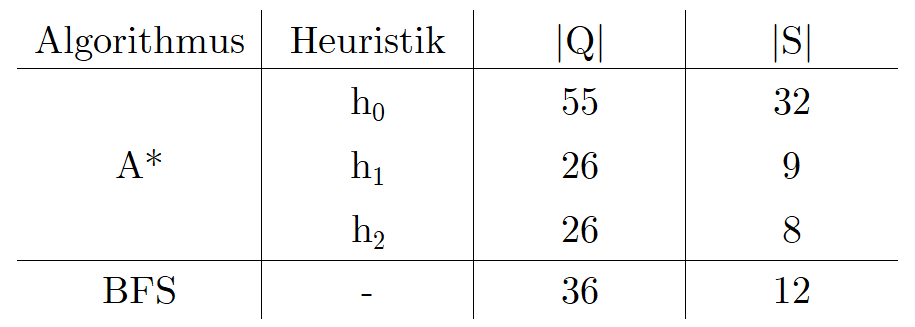
\includegraphics[width=0.6\linewidth]{figures/Q_S_Table.png}
\end{center}
Für den IDA*-Algorithmus wurden diese Werte in der Aufgabenstellung nicht gefordert und entsprechend auch nicht 
bei der Implementierung des IDA* umgesetzt.


\clearpage


\section{ Algorithmenprotokollierung }\label{se:protocol}
\paragraph*{}
Nachfolgend sind alle sieben Algorithmendurchführungen tabellarisch protokolliert. Wie in den Übungen entspricht
eine Tabelle der Durchführung eines Breitensuchenschritts im A*-Algorithmus und der BFS. Beim IDA*-Algorithmus 
sind aufgrund der Länge nur die Ergebnisse der iterativen, nicht aber der rekursiven, Schritte protokolliert.
\paragraph*{}
Zunächst ist zur Referenz der Graph, der die Springerzüge auf einem Schachbrett modelliert, als Adjazenzliste 
gegeben. Danach werden die tabellarischen Protokolle in der Reihenfolge
\begin{enumerate}
    \item A*, $h_0$
    \item A*, $h_1$
    \item A*, $h_2$
    \item BFS
    \item IDA* $h_0$
    \item IDA* $h_1$
    \item IDA* $h_2$
\end{enumerate}
angeführt.

\newpage
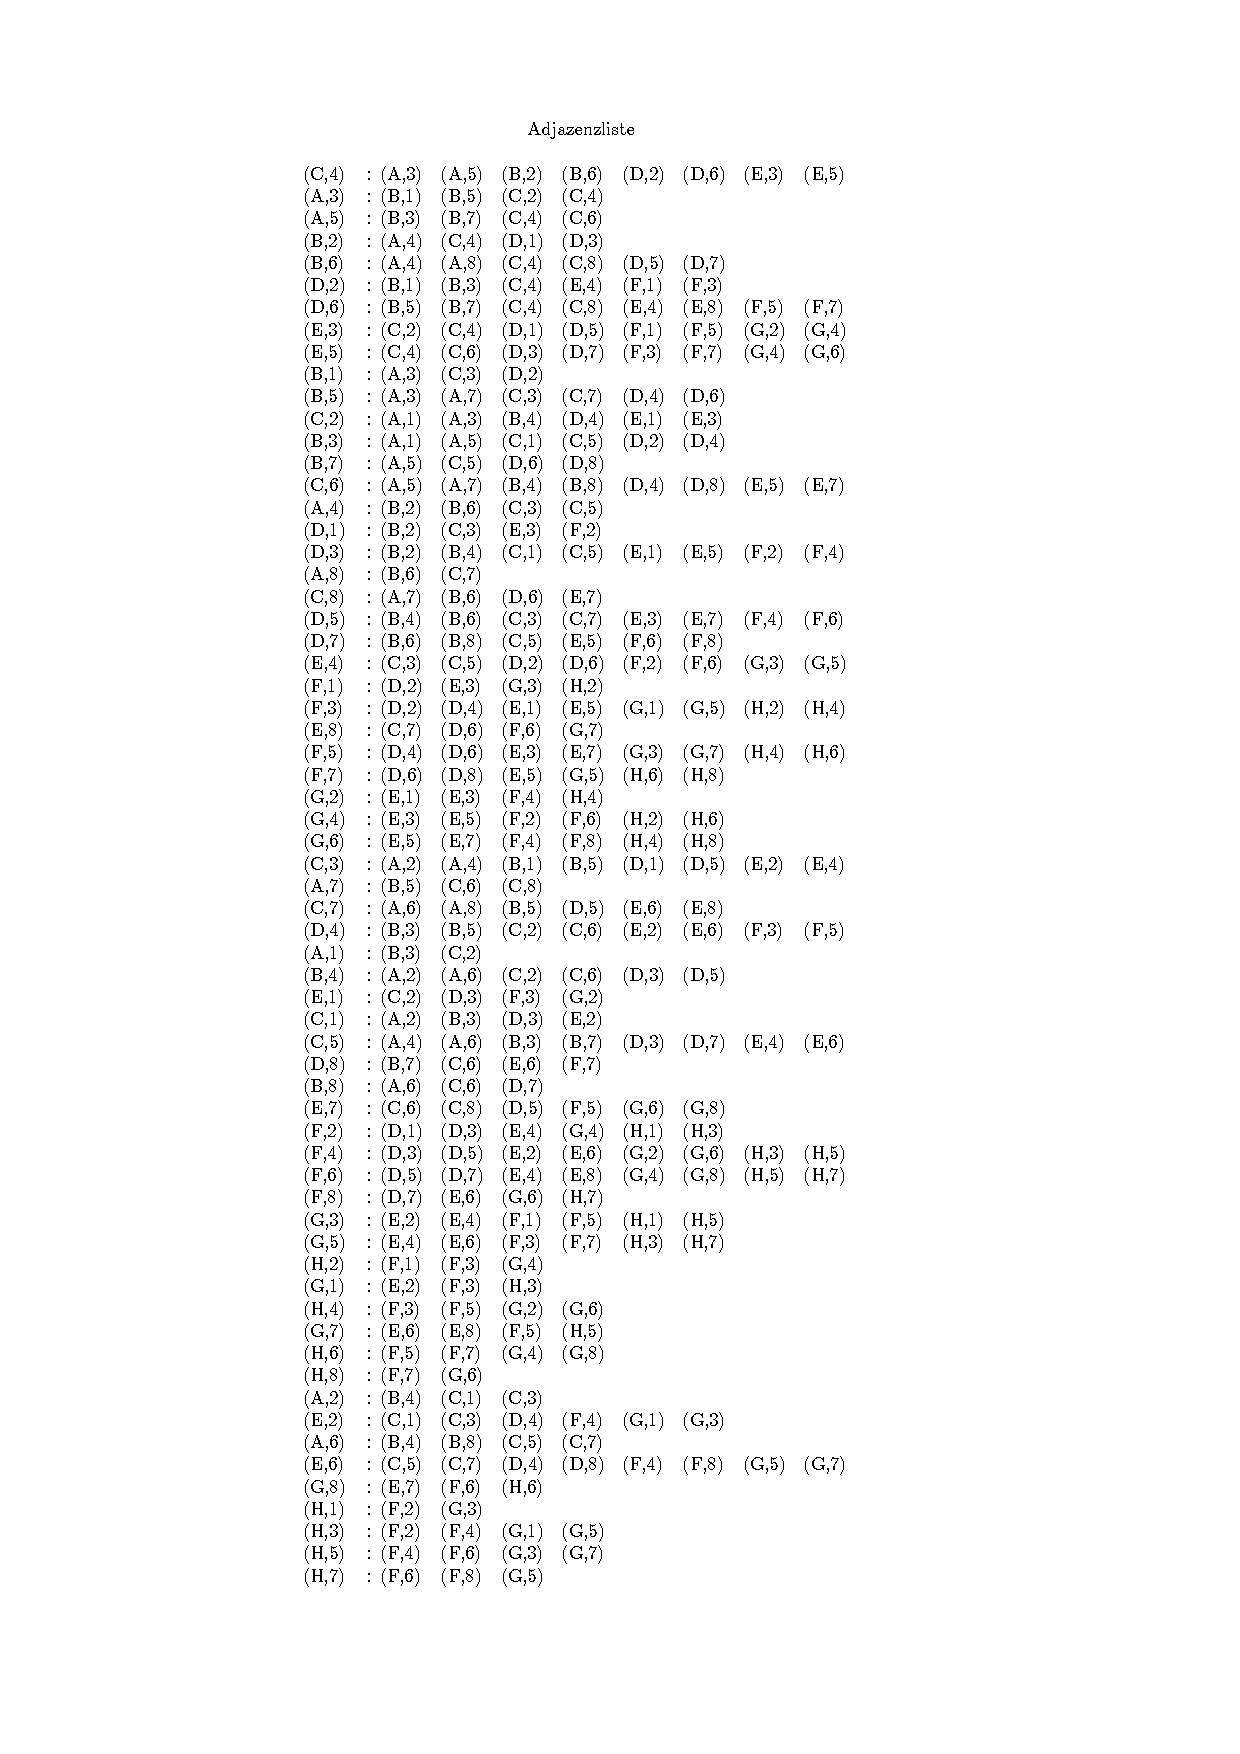
\includepdf{external_pdfs/graph.pdf}

\newpage
\huge

\vspace*{\fill}
\begin{center}
    A*, $h_0$ Protokoll
\end{center}
\vspace*{\fill}
\newpage
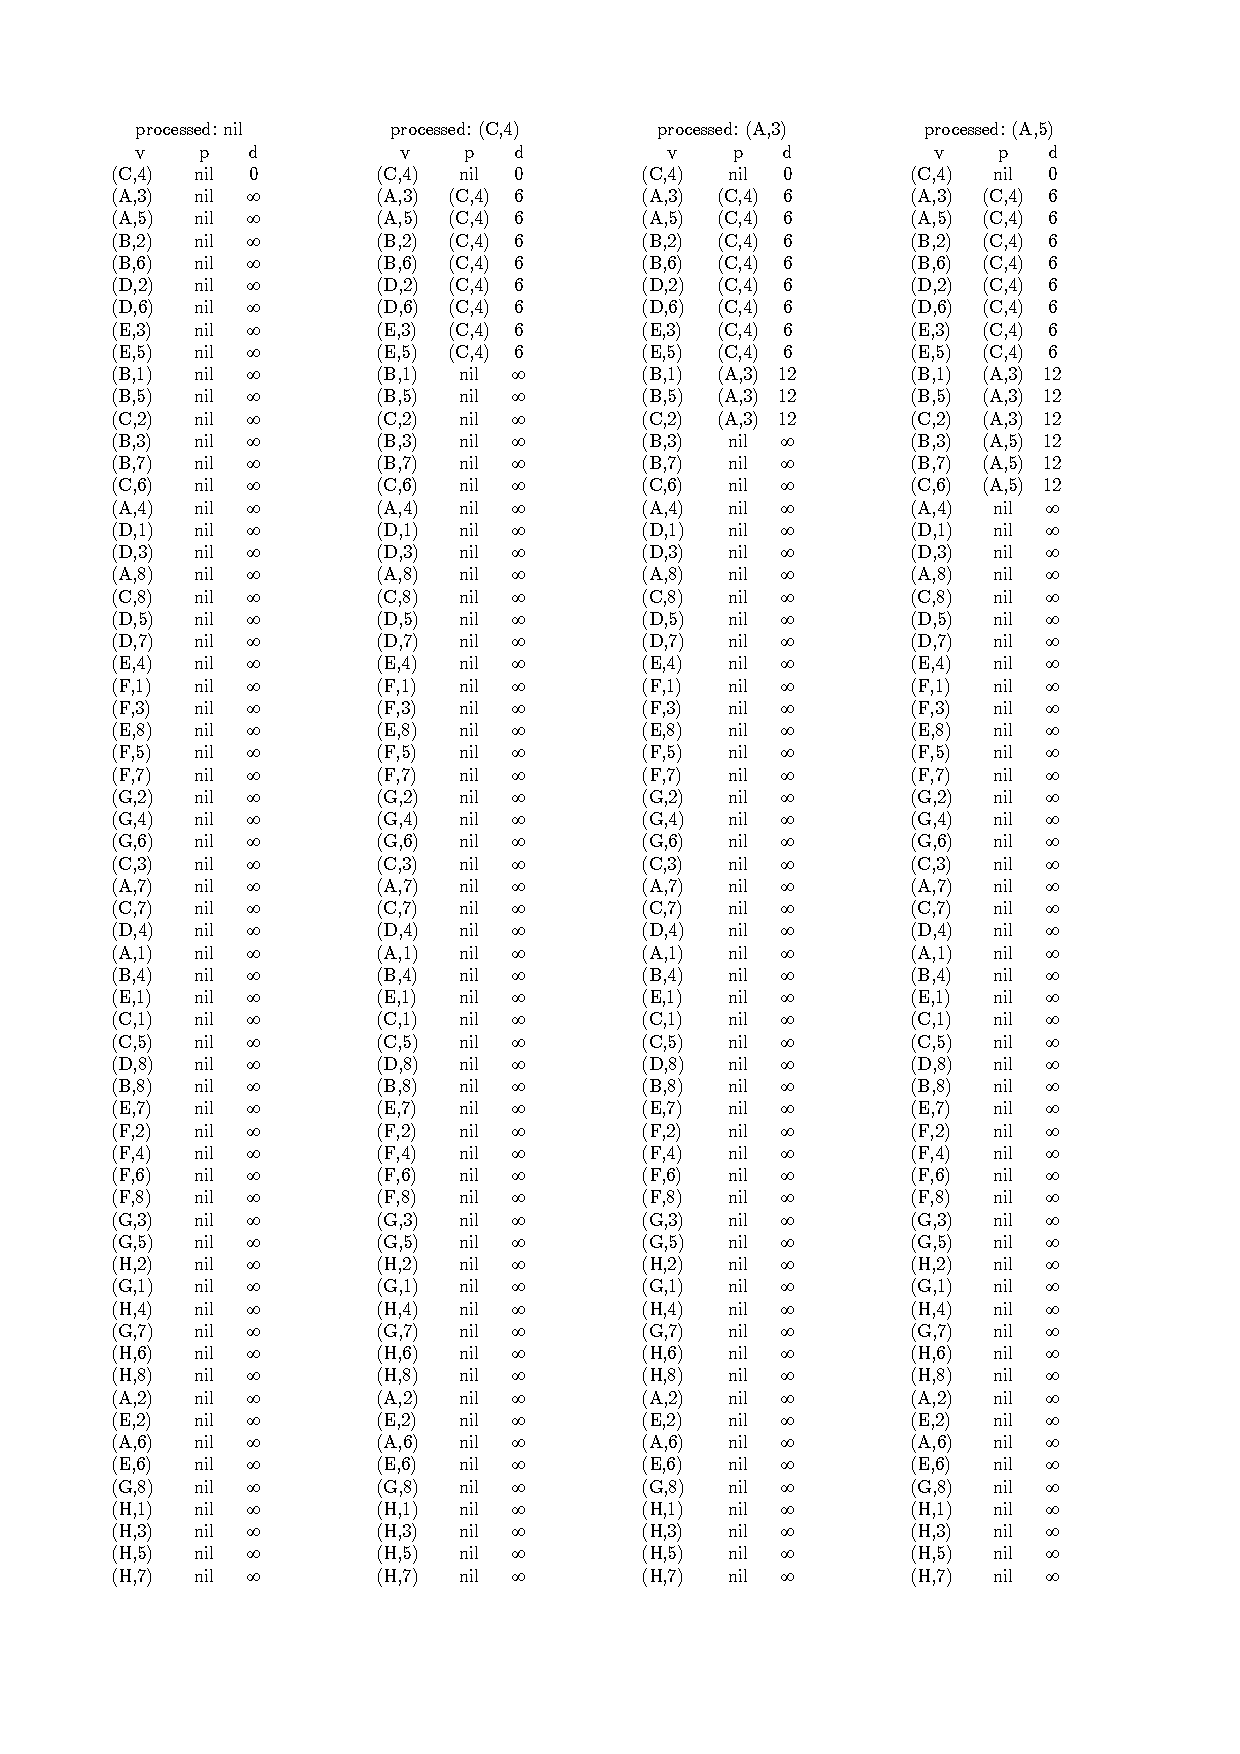
\includepdf{external_pdfs/astar_0.pdf}

\newpage
\vspace*{\fill}
\begin{center}
    A*, $h_1$ Protokoll
\end{center}
\vspace*{\fill}
\newpage
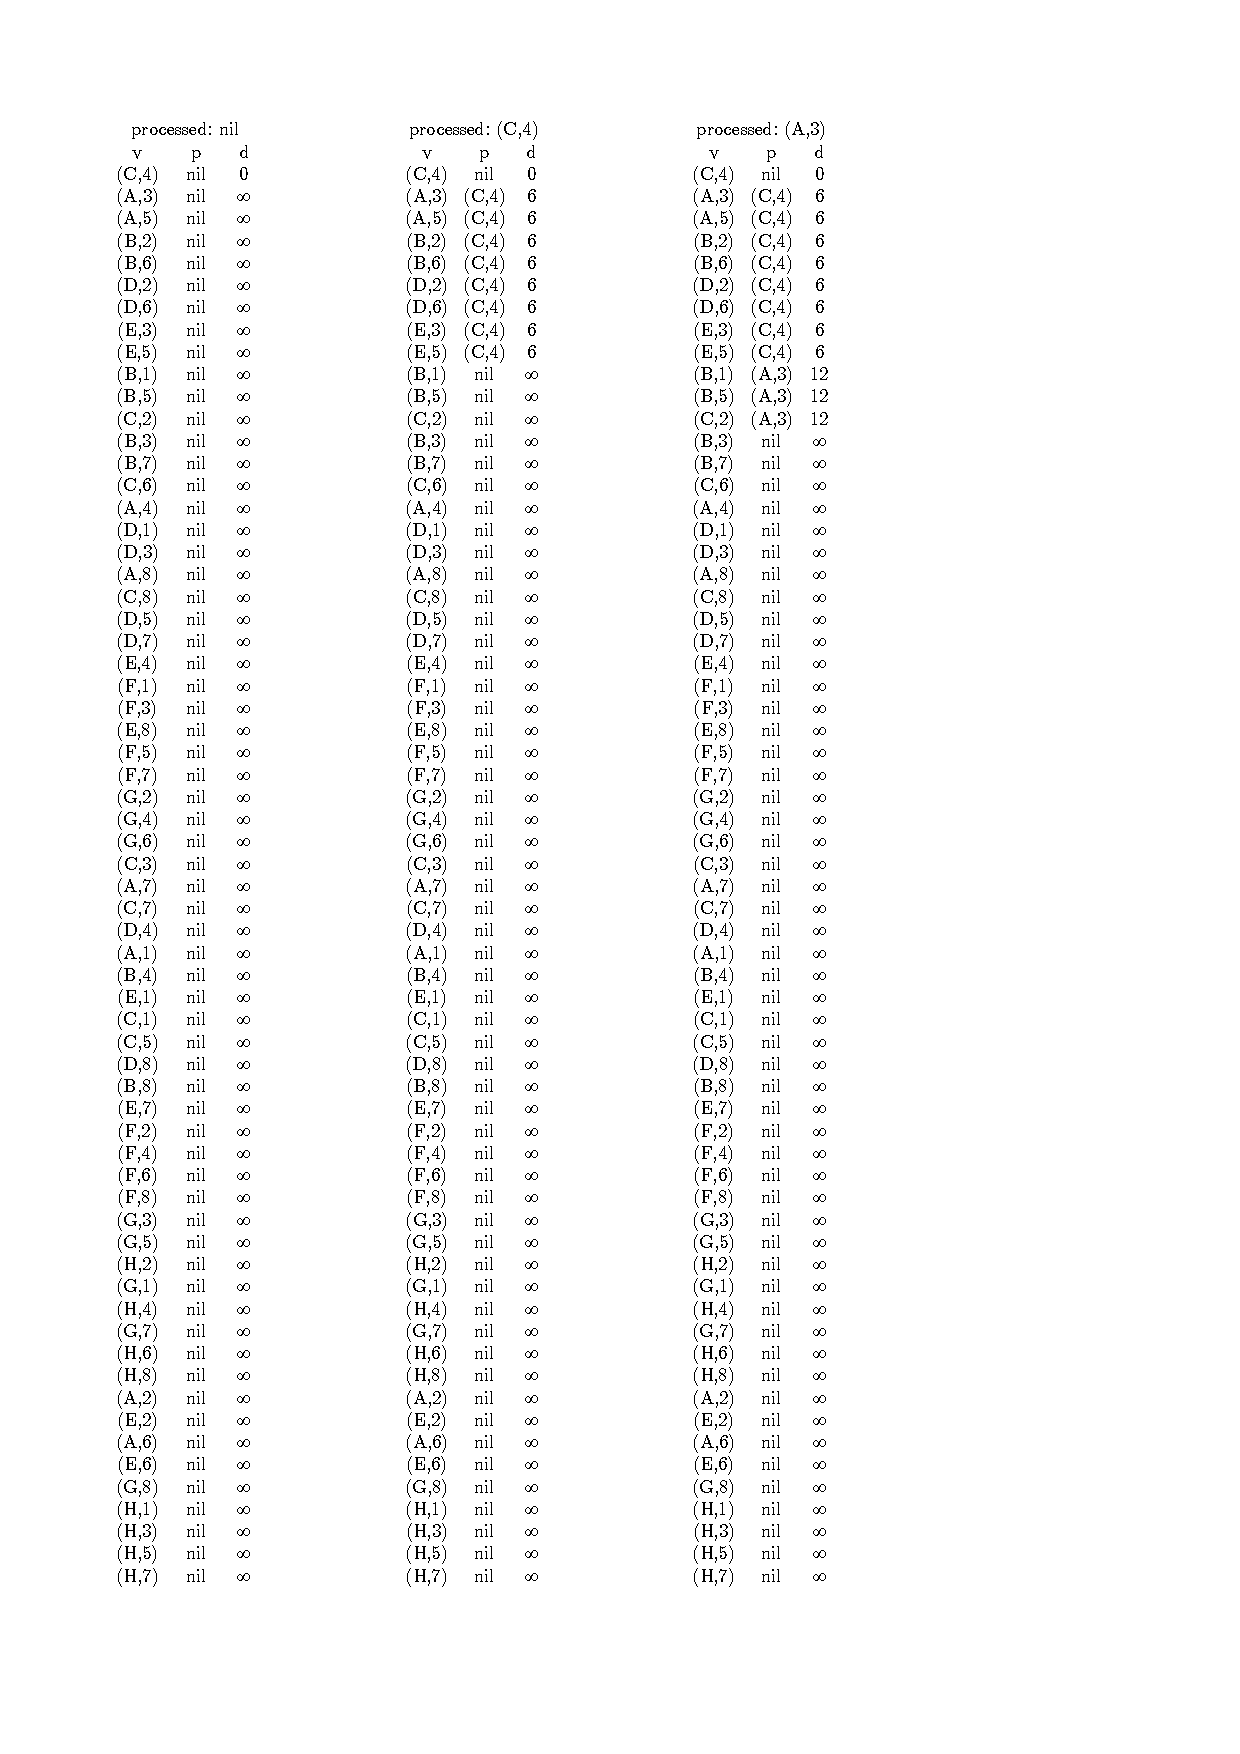
\includepdf{external_pdfs/astar_manhattendist.pdf}

\newpage
\vspace*{\fill}
\begin{center}
    A*, $h_2$ Protokoll
\end{center}
\vspace*{\fill}
\newpage
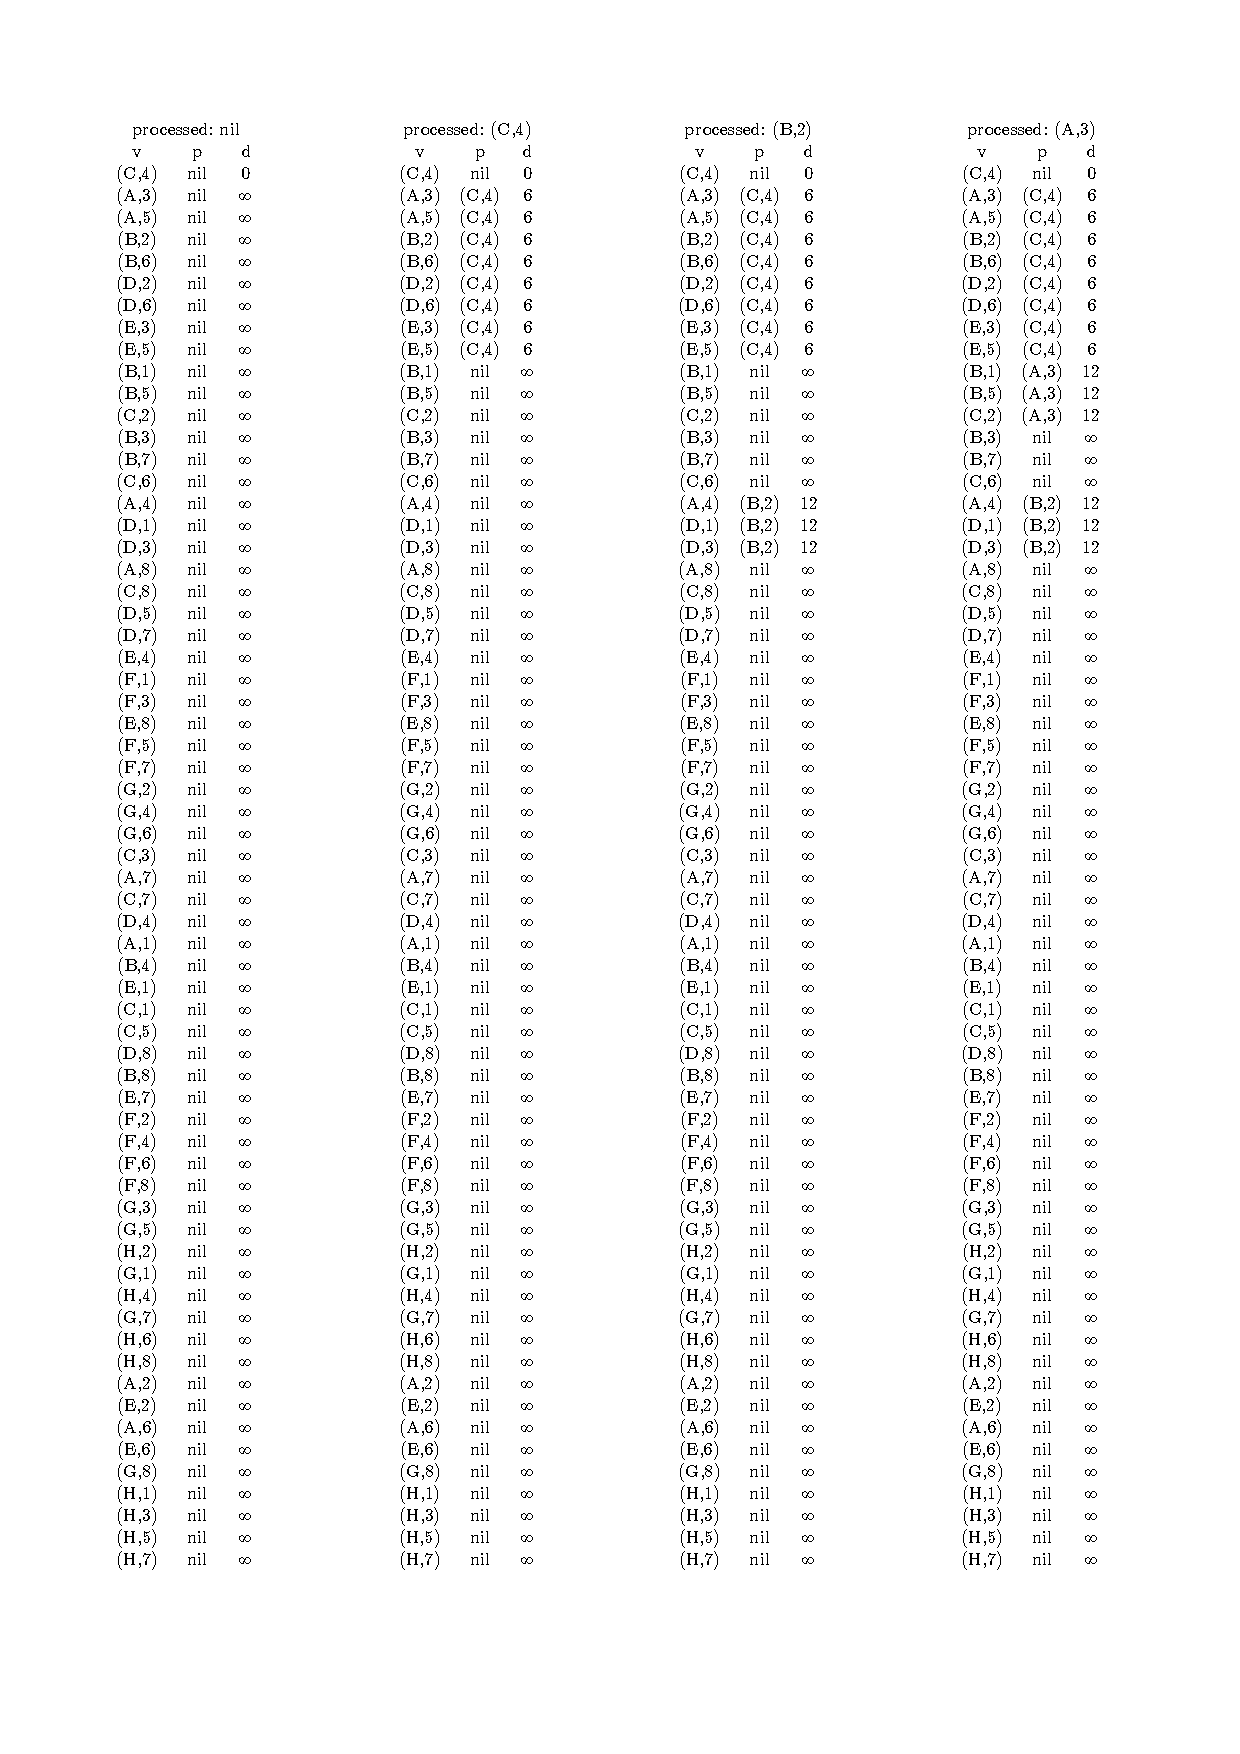
\includepdf{external_pdfs/astar_euclidmax.pdf}

\newpage
\vspace*{\fill}
\begin{center}
    BFS Protokoll
\end{center}
\vspace*{\fill}
\newpage
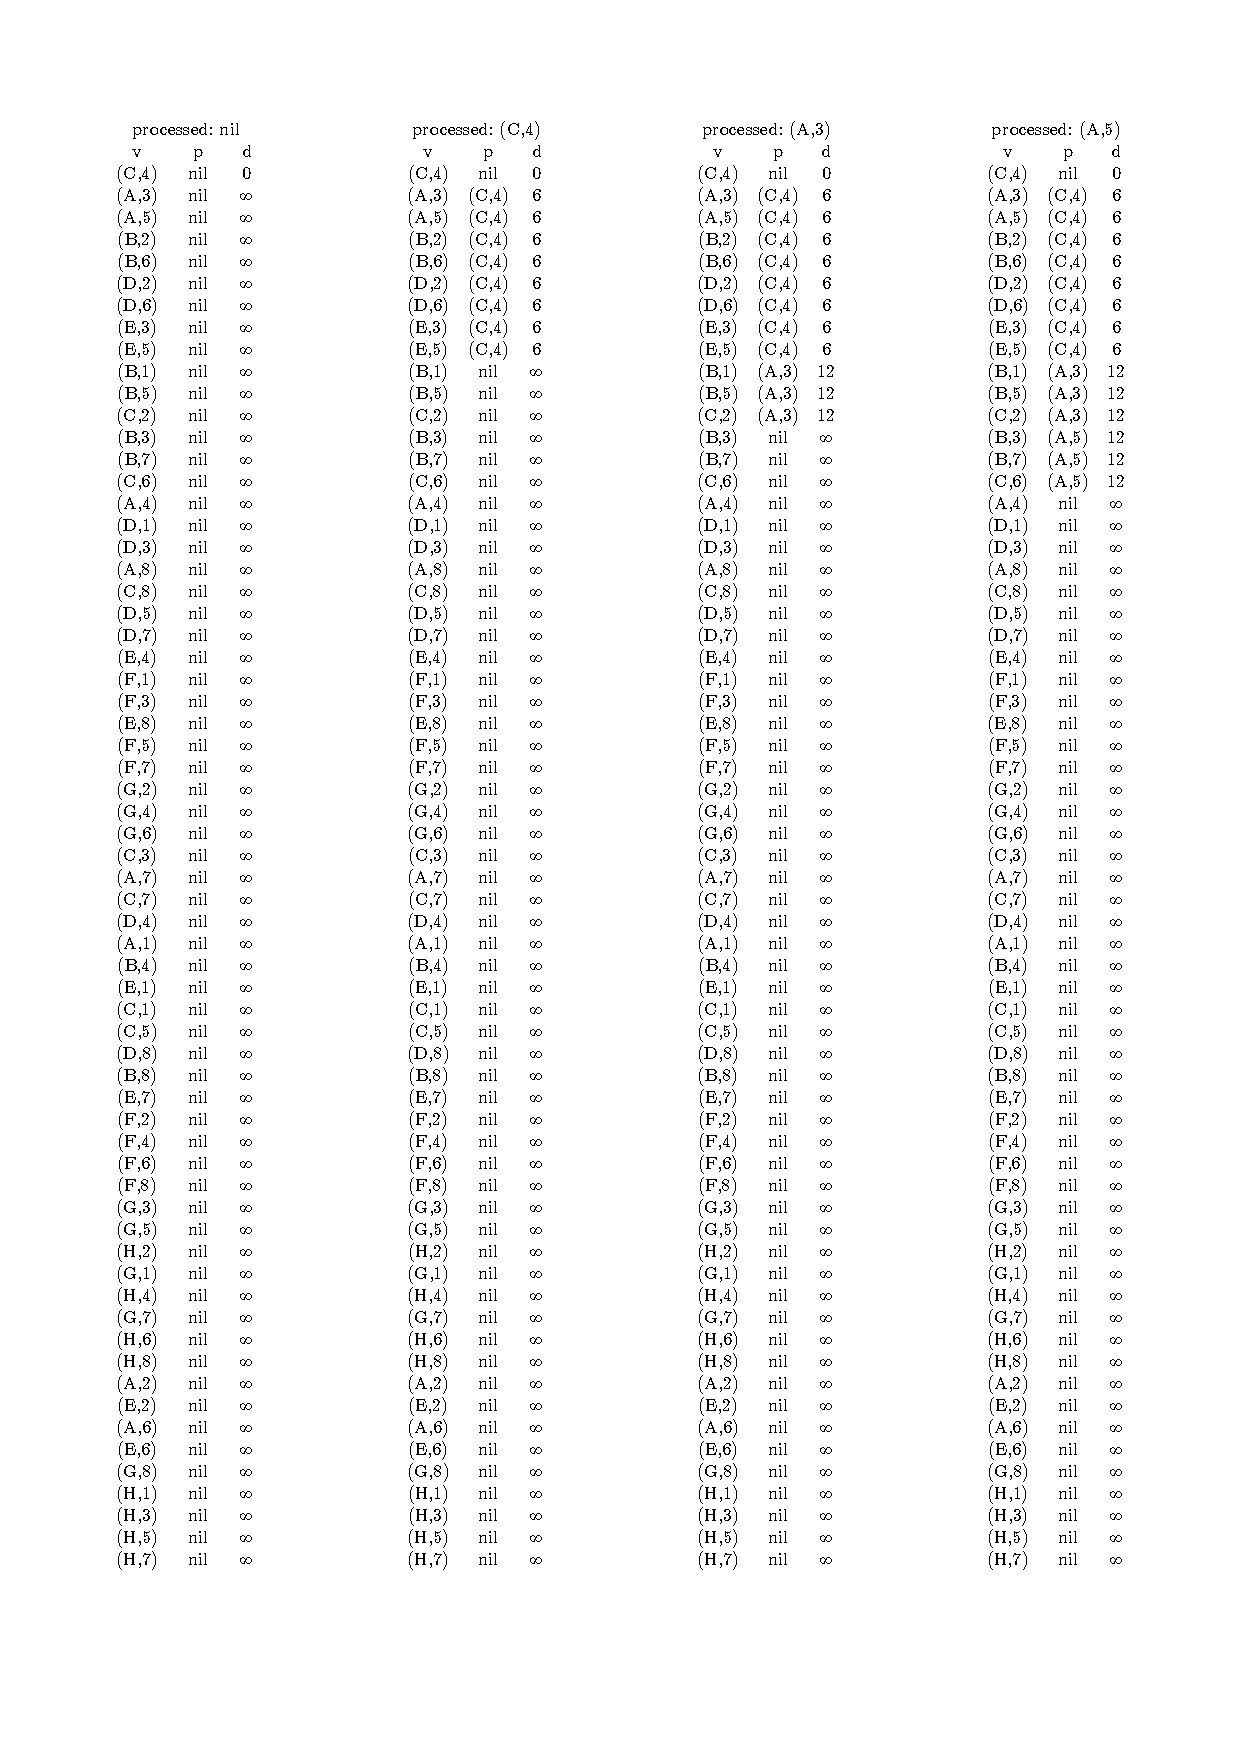
\includepdf{external_pdfs/bfs.pdf}

\newpage
\vspace*{\fill}
\begin{center}
    IDA*, $h_0$ Protokoll
\end{center}
\vspace*{\fill}
\newpage
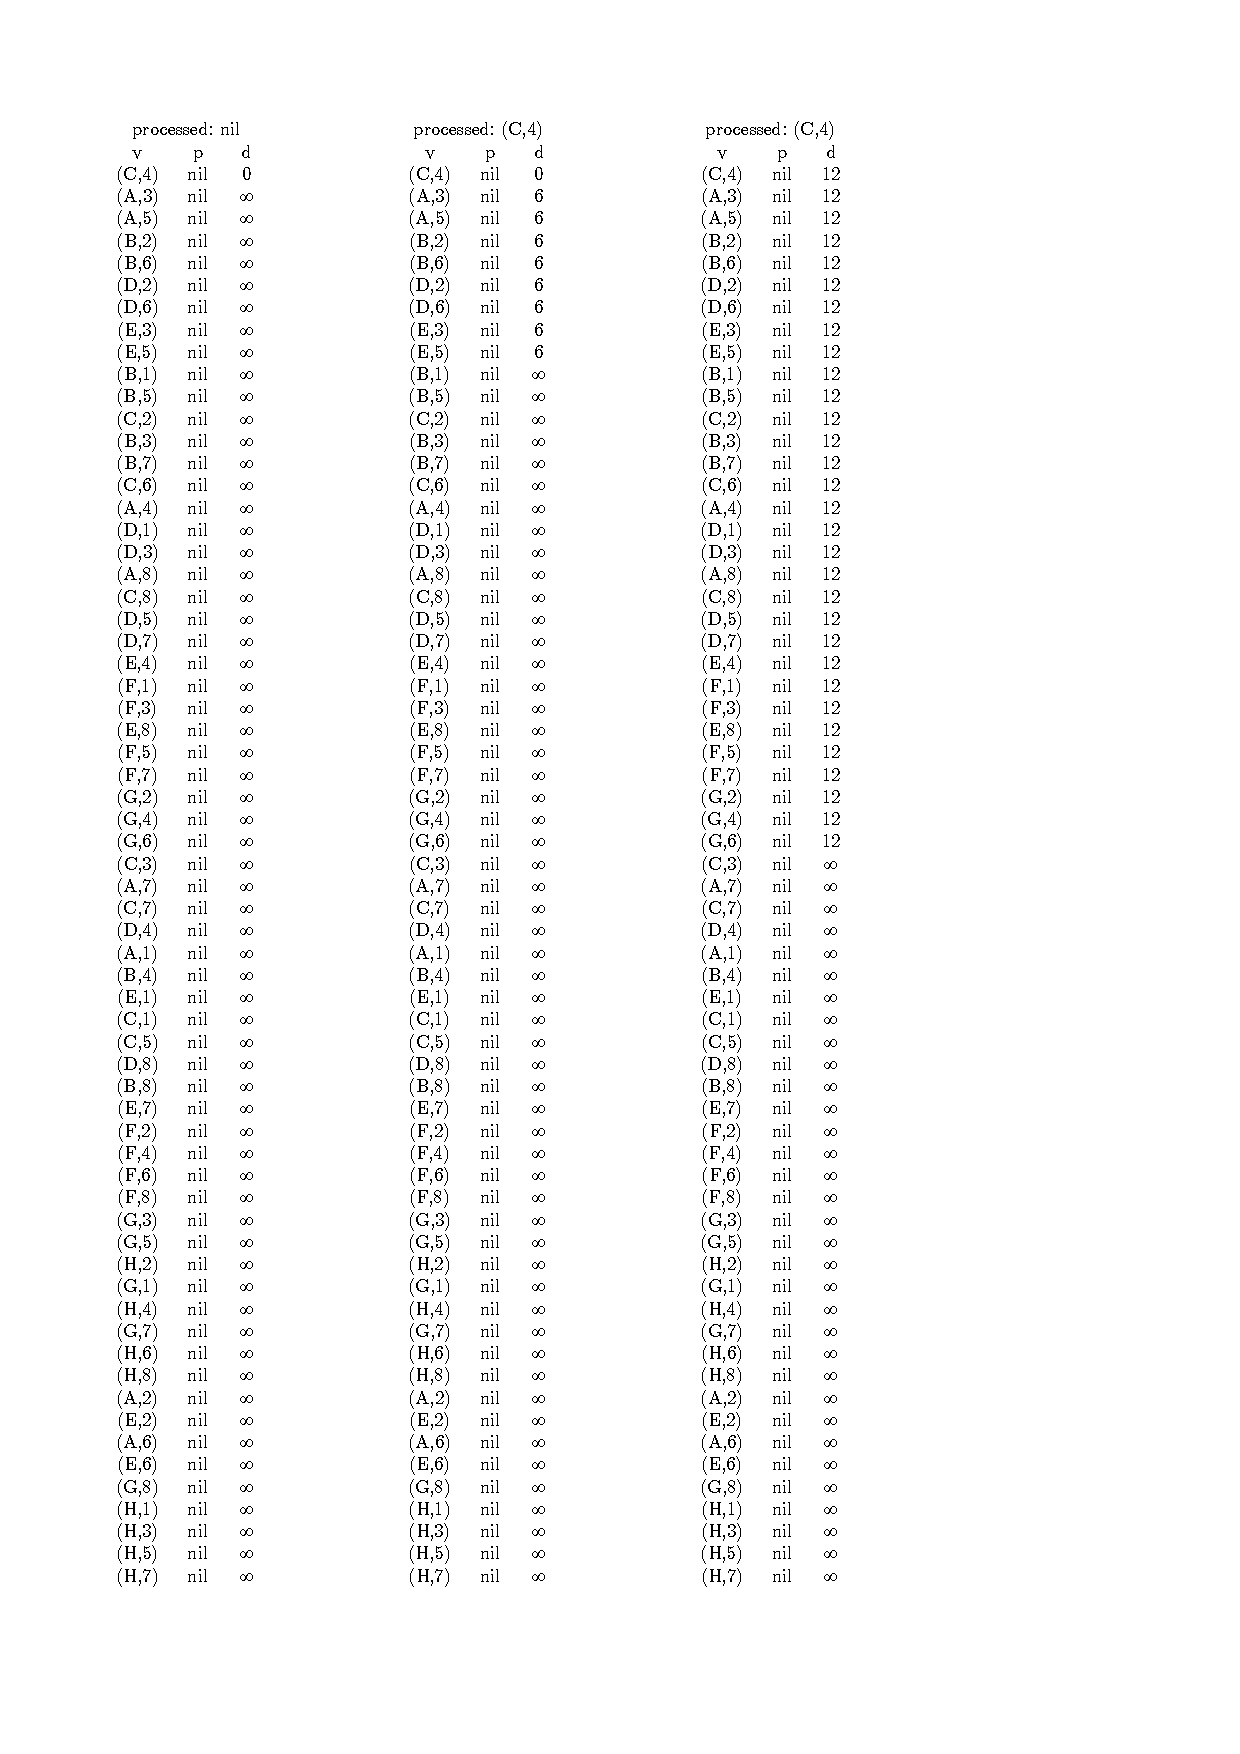
\includepdf{external_pdfs/idastar_0.pdf}

\newpage
\vspace*{\fill}
\begin{center}
    IDA*, $h_1$ Protokoll
\end{center}
\vspace*{\fill}
\newpage
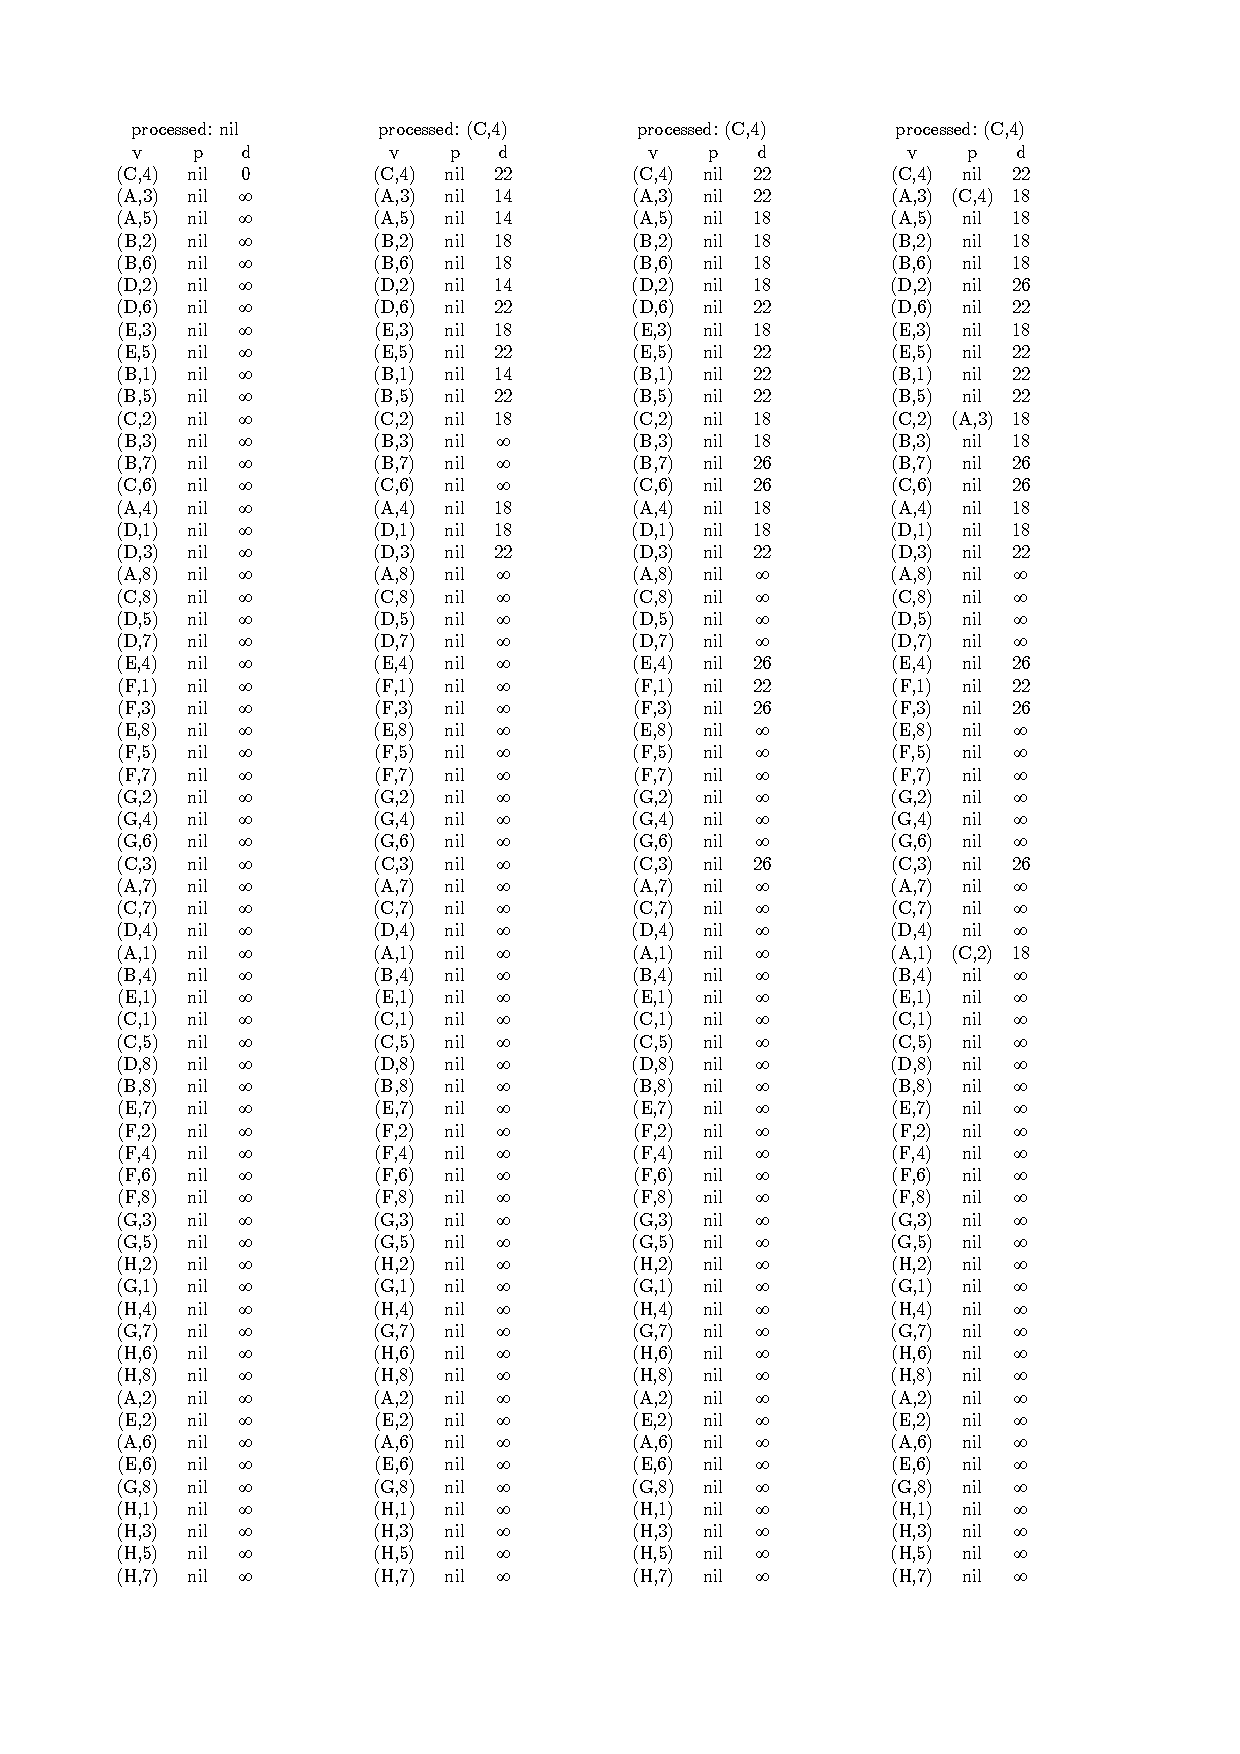
\includepdf{external_pdfs/idastar_manhattendist.pdf}

\newpage
\vspace*{\fill}
\begin{center}
    IDA*, $h_2$ Protokoll
\end{center}
\vspace*{\fill}
\newpage
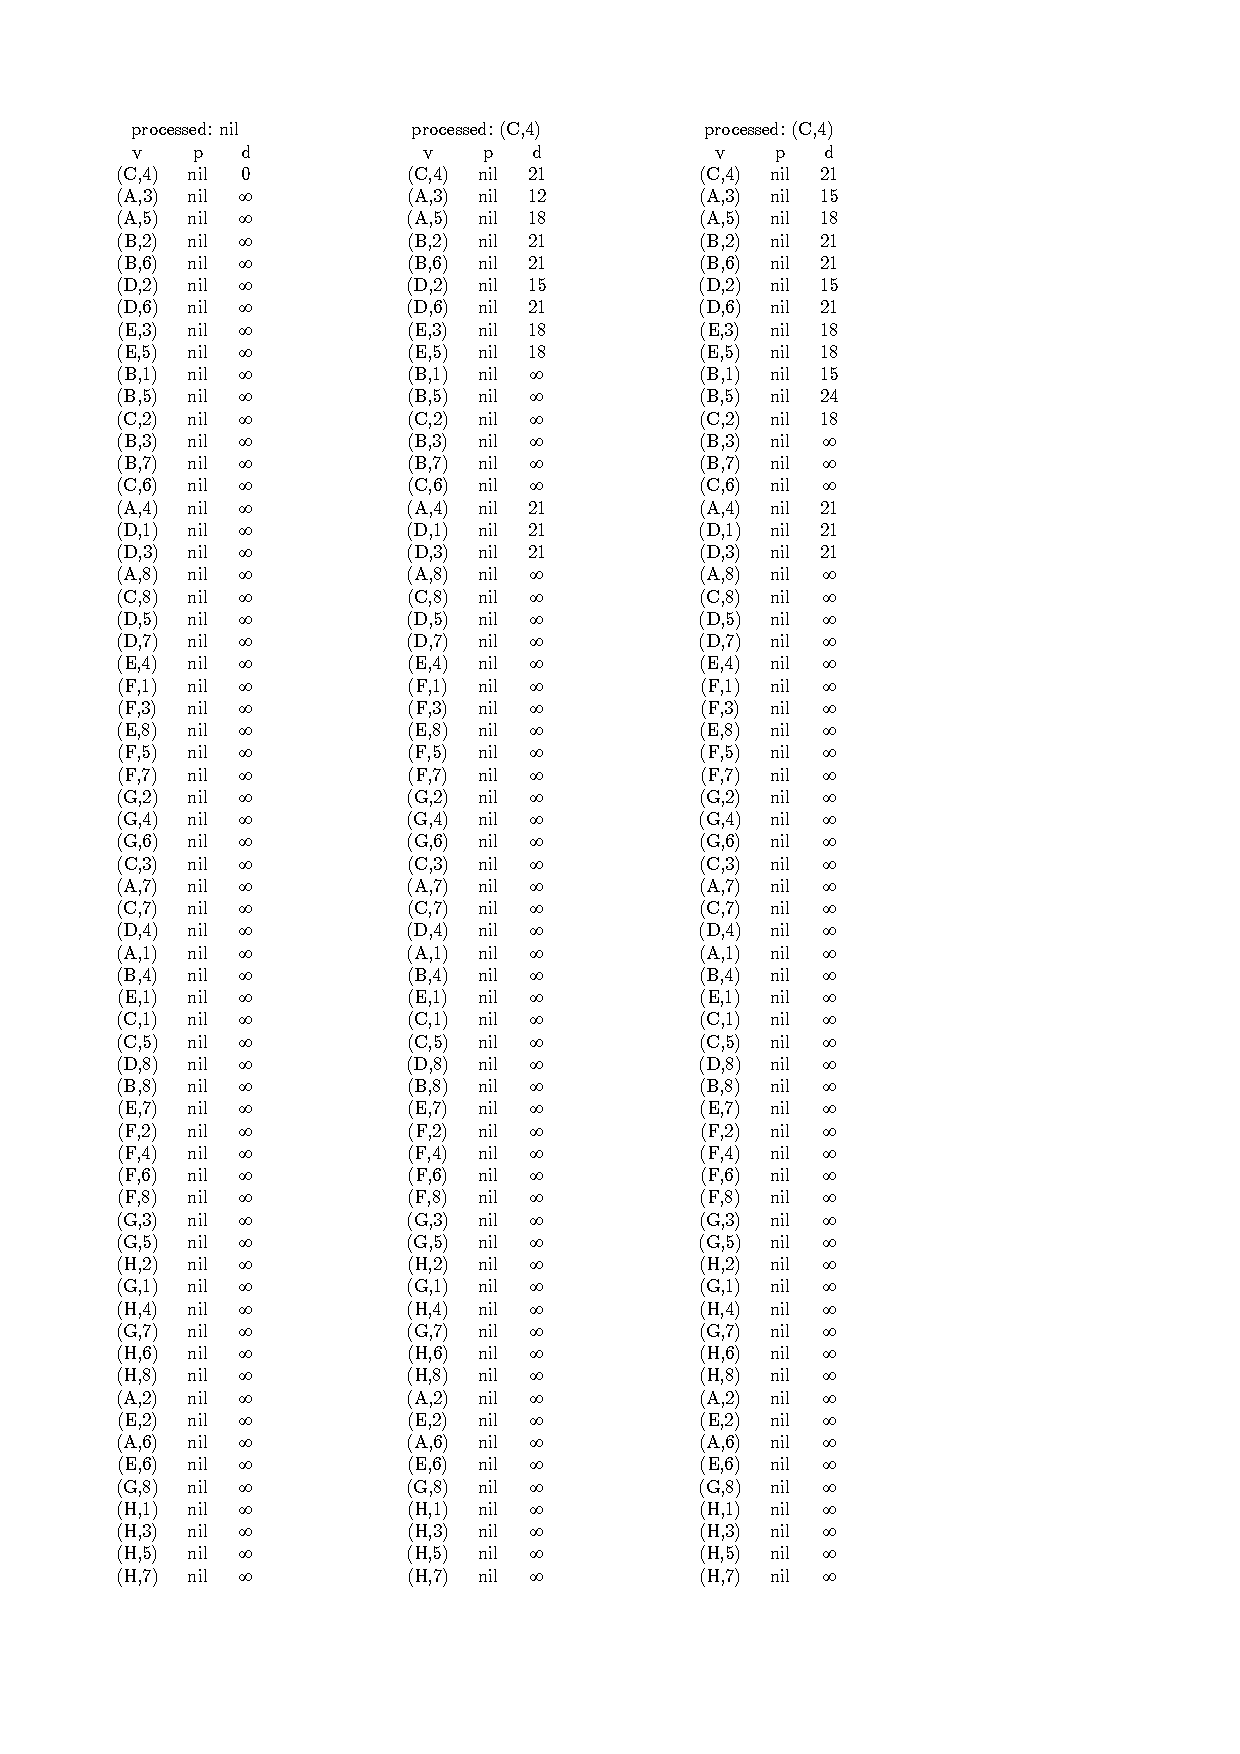
\includepdf{external_pdfs/idastar_euclidmax.pdf}
